\documentclass{beamer}
\begin{document}
    \begin{frame}
        \frametitle{Memcached}
        \begin{itemize}
            \item Web caching system developed by Firzpatrick for Livejournal.
            \item Several completely independent servers that store hashtables.
            \item A client chooses who to send a put/get.
        \end{itemize}
    \end{frame}
    \begin{frame}
        \frametitle{Drawbacks}
        \begin{itemize}
            \item If a server fails, one needs to reconfigure everything and invalidate
            all entries, or suffer from cache misses.
            \item If several entries are super popular, then the corresponding servers
            suffer from heavier load.
        \end{itemize}
    \end{frame}
    \begin{frame}
        \frametitle{Consistent Hashing}
        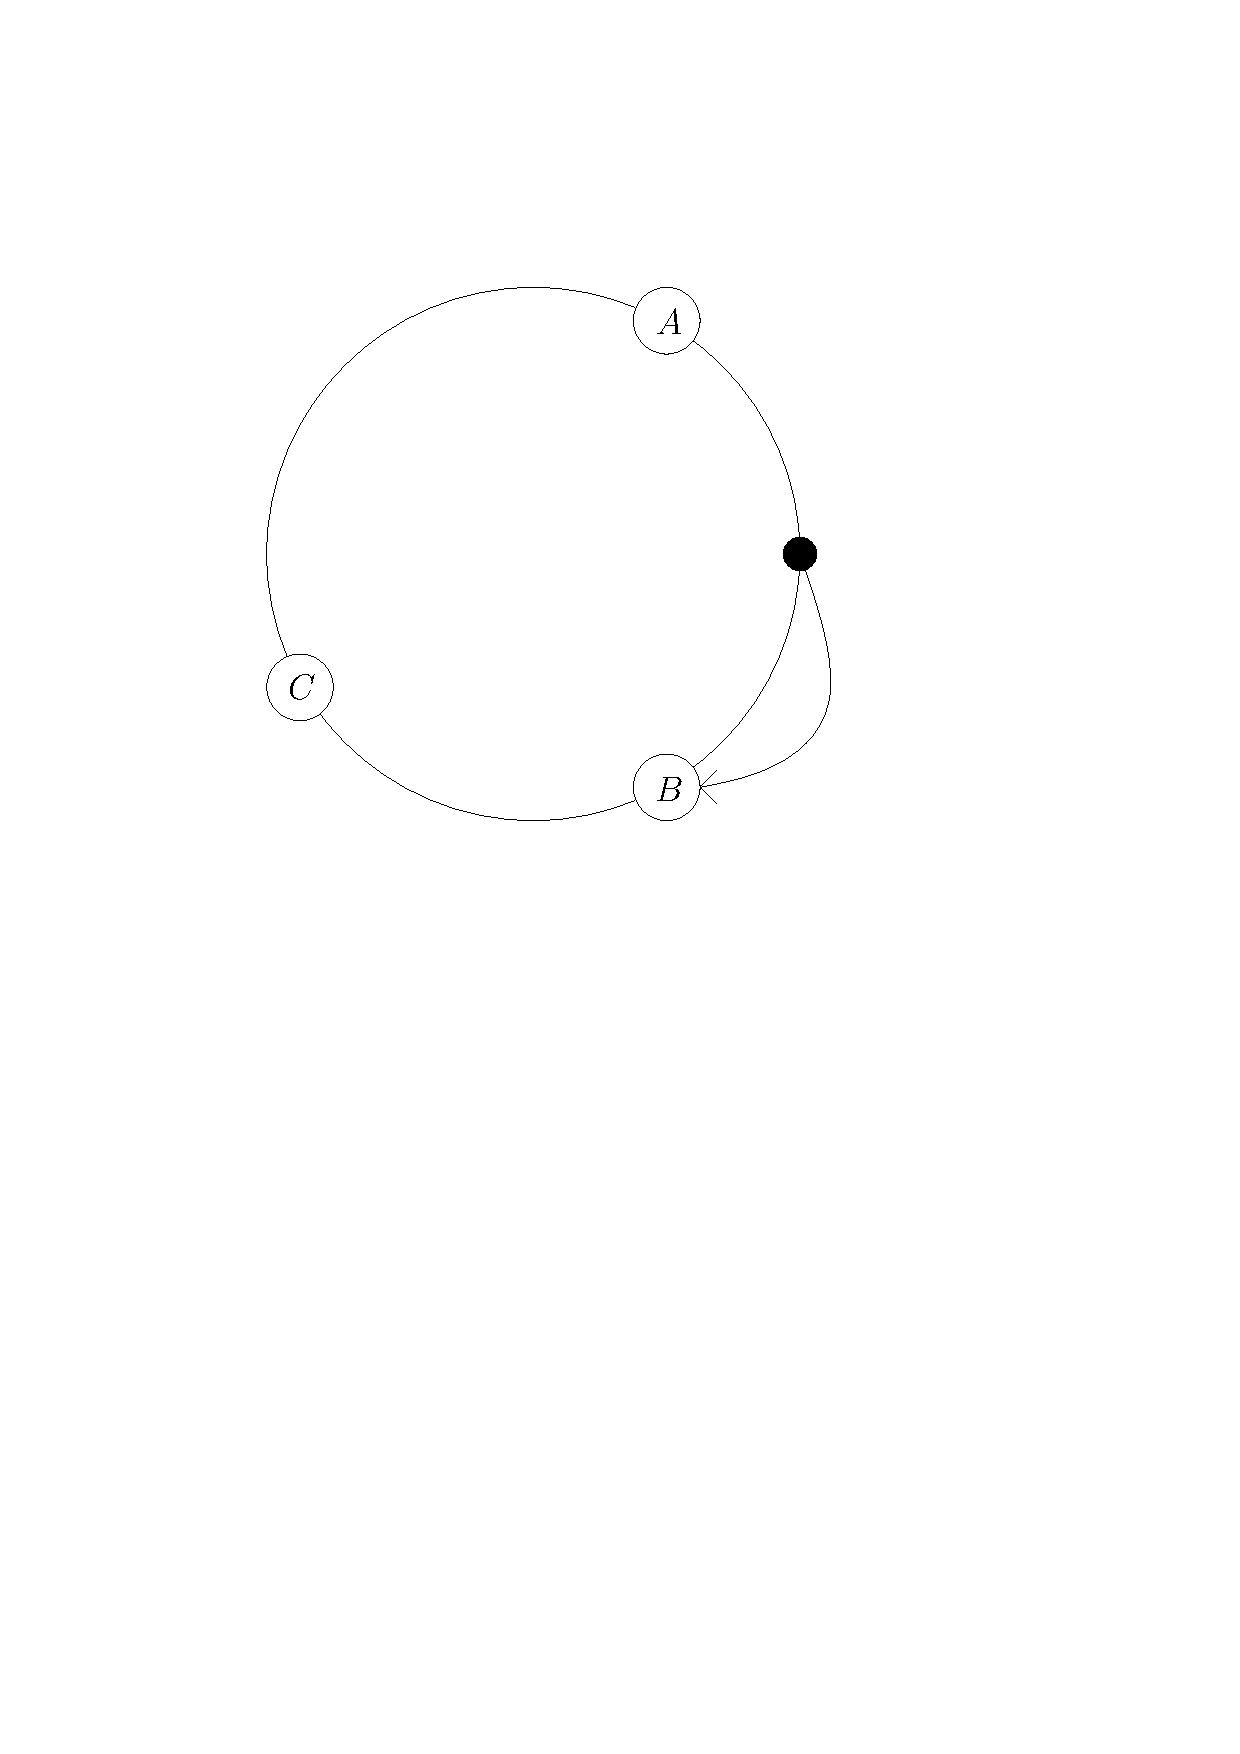
\includegraphics[scale=0.3]{hashing.pdf}
        \begin{itemize}
            \item Map keys to a circle using hashing, and then find a server that is responsible.
            \item View server tracks servers and is capable of reporting server-to-location mappings.
            \item If a server fails, then only $\approx 1/N$ fraction of keys is remapped.
            \item A view server is a single point of failure, but can be replicated using Paxos.
        \end{itemize}
    \end{frame}
    \begin{frame}
        \frametitle{Replication}
        \begin{itemize}
            \item Each server can be replicated.
            \item A client can read or write using \emph{any} server.
            \item From time to time servers do anti--entropy sessions in order to sync data.
            \item Provides a weak consistency model, but good enough, if data is accessed frequently, but updated
            sporadically.
        \end{itemize}
    \end{frame}
    \begin{frame}
      \frametitle{Performance}
      \begin{itemize}
        \item Basic setup: 5 servers and view service on one machine, 40 clients across two other machines
        \item Stress test: Clients perform random put/get operations as fast as possible
        \item Throughput of 40000 operations/second
        \item Test 1: 5 additional servers on another machine
        \item Throughput increases to 60000 operations/second
        \item Test 2: 5 additional servers on another machine, mirroring original 5
        \item Throughput increases to 70000 operations/second
      \end{itemize}
    \end{frame}
\end{document}
